\documentclass[10pt,a4paper,twocolumn]{article}
\usepackage[T1]{fontenc}
\usepackage[utf8]{inputenc}
\usepackage{anysize, longtable}
\usepackage{amsthm, amsfonts, amsmath, amssymb, booktabs, float}
\usepackage{sectsty, csquotes, xcolor, xspace, setspace, listings}
\usepackage{graphicx, tabularx, changepage, multirow, subcaption}
\usepackage{algorithm, algpseudocode, multicol, cuted, colortbl}
\usepackage{makecell, supertabular}
\usepackage[hidelinks,bookmarksdepth=3]{hyperref}
\usepackage[capitalise]{cleveref}
\usepackage[inline]{enumitem}
\usepackage[english]{babel}
\usepackage{microtype}
\usepackage{libertinus}
\usepackage[scale = 0.85]{plex-mono}
\usepackage[maxbibnames=99]{biblatex}
\usepackage{titlesec}
\usepackage{tikz}

\usetikzlibrary{fit, shapes.geometric, shapes.symbols, positioning, shapes.misc, calc, arrows.meta, patterns, backgrounds, decorations, decorations.markings, decorations.pathreplacing, shadows, hobby, decorations.pathmorphing}

\makeatletter

\theoremstyle{plain}
\newtheorem{theorem}{Theorem}
\newtheorem{lemma}{Lemma}

\theoremstyle{definition}
\newtheorem{definition}{Definition}
\newtheorem{example}{Example}

\theoremstyle{remark}
\newtheorem*{note}{Note}
\newtheorem*{remark}{Remark}

\newcommand{\inlinecode}[1]{\lstinline[basicstyle=\ttfamily,columns=fixed]$#1$}
\lstset{basicstyle=\setstretch{0}\small\ttfamily,breaklines=true,columns=fixed,captionpos=b,xleftmargin=0.5cm}

\newlength{\offsetpage}
\newenvironment{widepage}[1][2cm]{
  \setlength{\offsetpage}{#1}
  \begin{adjustwidth}{-\offsetpage}{-\offsetpage}
  \addtolength{\linewidth}{2\offsetpage}
}{\end{adjustwidth}}

\algnewcommand{\IIf}[1]{\State \algorithmicif\ #1\ \algorithmicthen}
\algnewcommand{\IElse}[1]{\algorithmicelse\ #1}
\algnewcommand{\EndIIf}{\unskip\ \algorithmicend\ \algorithmicif}

\addbibresource{biblio.bib}

\allowdisplaybreaks
\marginsize{2.0cm}{2.0cm}{1.25cm}{1.25cm}
\setcounter{tocdepth}{2}
\setlist[itemize]{topsep=0pt, partopsep=0pt, parsep=0pt, itemsep=\parskip}
\setlist[enumerate]{topsep=0pt, partopsep=0pt, parsep=0pt, itemsep=\parskip}
\titlespacing*{\paragraph}{0pt}{0.5\baselineskip}{0.5\baselineskip}
\captionsetup[figure]{aboveskip=5pt}
\captionsetup[subfigure]{aboveskip=3pt}

\title{Real-Time Analysis of Public GitHub Activity}
\author{Roland Bernard, 19598, \inlinecode{rolbernard@unibz.it}}
\date{February 2026}

\def\maketitle{
\begin{strip}
  \begin{adjustwidth}{5mm}{5mm}
    \vspace{-4.5em}
    \noindent{\small\bfseries Project Report -- Real-Time Big Data Processing 2024/2025\par}
    \vskip 0.25em
    \noindent{\LARGE\bfseries \@title\par}
    \vskip 1em
    \noindent{\large \@author\par}
    \vskip 1em
    \noindent{\small \@date\par}
    \vskip 2em
    \noindent{
      \small
      \begin{tabular}{rl}
        Code Repository & \url{https://gitlab.inf.unibz.it/Roland.Bernard/rtbdp-project}, or \\
                        & \url{https://github.com/rolandbernard/rtbdp-project} \\
        Commit & TODO (latest commit in the repository) \\
        Live Demo Link & \url{https://rtgh.rolandb.com/} \\
      \end{tabular}
    }
    \vskip 1em
  \end{adjustwidth}
\end{strip}
}
\renewenvironment{abstract}{
  \vskip 1em
  \begin{quote}
  {\normalsize \abstractname\par}
  \small
}{
  \end{quote}
  \vskip 1em
}

\makeatother

\definecolor{unibzblue}{HTML}{0086ec}
\definecolor{unibzblue2}{HTML}{f0f8ff}

\pgfdeclarelayer{background}
\pgfdeclarelayer{foreground}
\pgfsetlayers{background,main,foreground}

\tikzset{
  flow/.style={-{Triangle[length=6, width=6]}, draw=red!70!black, very thick, shorten >= -3},
  biflow/.style={flow, {Triangle[length=6, width=6]}-{Triangle[length=6, width=6]}},
  link/.style={->, draw},
  ptr/.style={->, dashed},
  leafl/.style={-, thick},
  external/.style={inner sep=10, draw=black, fill=brown!20},
  internal/.style={inner sep=10, draw=black, fill=unibzblue!20},
  build/.style={inner sep=10, draw=black, fill=unibzblue!40},
  mixed/.style={inner sep=8.7, draw=black, path picture={
    \fill[brown!20] (path picture bounding box.south west)
      rectangle ($(path picture bounding box.north west)!.675!(path picture bounding box.north east)$);
    \fill[unibzblue!40] ($(path picture bounding box.north west)!.675!(path picture bounding box.north east)$)
      rectangle (path picture bounding box.south east);
  }},
  >=Latex, node distance=1, every node/.style={inner sep=0}
}


\begin{document}

\maketitle

\begin{abstract}
Lorem ipsum dolor sit amet, consectetur adipiscing elit. Donec nisi risus, suscipit sed mattis non, sagittis sed nisi. Sed a lobortis odio, quis dapibus nisl. Class aptent taciti sociosqu ad litora torquent per conubia nostra, per inceptos himenaeos. Fusce tincidunt sapien eu dolor ullamcorper, quis dapibus lectus venenatis. Nunc a blandit massa. Fusce ac fringilla nibh, nec eleifend mauris. Sed maximus tempus nibh, porta cursus mi rutrum et. Nunc erat massa, commodo id ornare ut, scelerisque ac est. Cras elit metus, aliquet sit amet maximus in, gravida in mauris. Vestibulum ante ipsum primis in faucibus orci luctus et ultrices posuere cubilia curae; Ut enim tellus, ornare quis malesuada non, scelerisque a elit. Donec dictum velit eu dui hendrerit ultrices. Pellentesque posuere porta odio eu feugiat.

Lorem ipsum dolor sit amet, consectetur adipiscing elit. Donec nisi risus, suscipit sed mattis non, sagittis sed nisi. Sed a lobortis odio, quis dapibus nisl. Class aptent taciti sociosqu ad litora
\end{abstract}


\section{Application Domain} \label{application}





\section{Description of the Data Sources} \label{dataset}

\subsection{GitHub Events API}

\subsection{Dummy API and GHArchive}

\subsection{Data Characteristics}



\section{\texorpdfstring{Technologies and \\Overall Architecture}{Technologies and Overall Architecture}} \label{architecture}

\subsection{Technology Stack}

\paragraph{Backend Components}
The backend services, i.e., the producer, the frontend server, and the Flink based processor, are implemented in Java \cite{java21}. Apache Maven \cite{mavenDocs} is used for dependency management and as a build system. Both the producer and the frontend server rely on RxJava \cite{rxJavaDocs} for reactive stream processing and managing asynchronous operations. In all backend components the Argparse4j library \cite{argparse4jDocs} is used to handle command-line configuration, while Jackson \cite{jacksonDocs} is utilized for high-performance JSON parsing. Logging is standardized by using SLF4J \cite{slf4jDocs} and Logback \cite{logbackDocs}, with JUnit \cite{junitDocs} used for unit testing to ensure code reliability.

\paragraph{Frontend Client}
The user interface of the project is implemented as a Single Page Application (SPA) built with TypeScript \cite{tsDocs} and React \cite{reactDocs}. Vite \cite{viteDocs} is used to serve as the build toolchain. React Router \cite{reactRouterDocs} is used to handle client-side routing. Styling is handled via Tailwind CSS \cite{tailwindDocs}, and data visualization is powered by the React based Recharts \cite{rechartsDocs} library. Communication with the backend utilizes RxJS \cite{rxjsDocs} to manage WebSocket streams and simple stream operations.

\paragraph{Stream Processing and Storage}
Further, the project makes use of a number of different technologies for the storage, processing, and streaming transmission of data. Firstly, Apache Kafka \cite{kafkaDocs,kreps2011kafka} is used as the central system for data ingestion and messaging in the project. Next, Kafka Flink \cite{flinkDocs,carbone2015apache} serves as the core stream processing engine in the project. Flink has been configured to utilize the RocksDB \cite{rocksdbDocs} state backend to manage large state sizes and enable fault tolerance. Flink is further configured for high availability, by using Apache ZooKeeper \cite{zookeeperDocs}. To provide persistent storage for processed data, the project uses PostgreSQL \cite{postgresDocs}, a popular open-source database management system. The project also uses the TimescaleDB extension \cite{timescaleDocs}, providing facilities for managing time-series data, especially partitioning and retention. Finally, the project makes use of Docker \cite{dockerDocs} and Docker Compose \cite{dockerCompose} to orchestrate all the services.

\subsection{System Architecture and Data Flow}

The project is built on a variation of the provided reference architecture. \Cref{fig:arch} shows an overview of the overall system architecture with all important components. The system follows a modular architecture, orchestrated via Docker Compose. The workflow is divided into four distinct stages, data ingestion, stream processing, data serving, and display of the results in the frontend.

\begin{figure*}[ht]
  \centering
  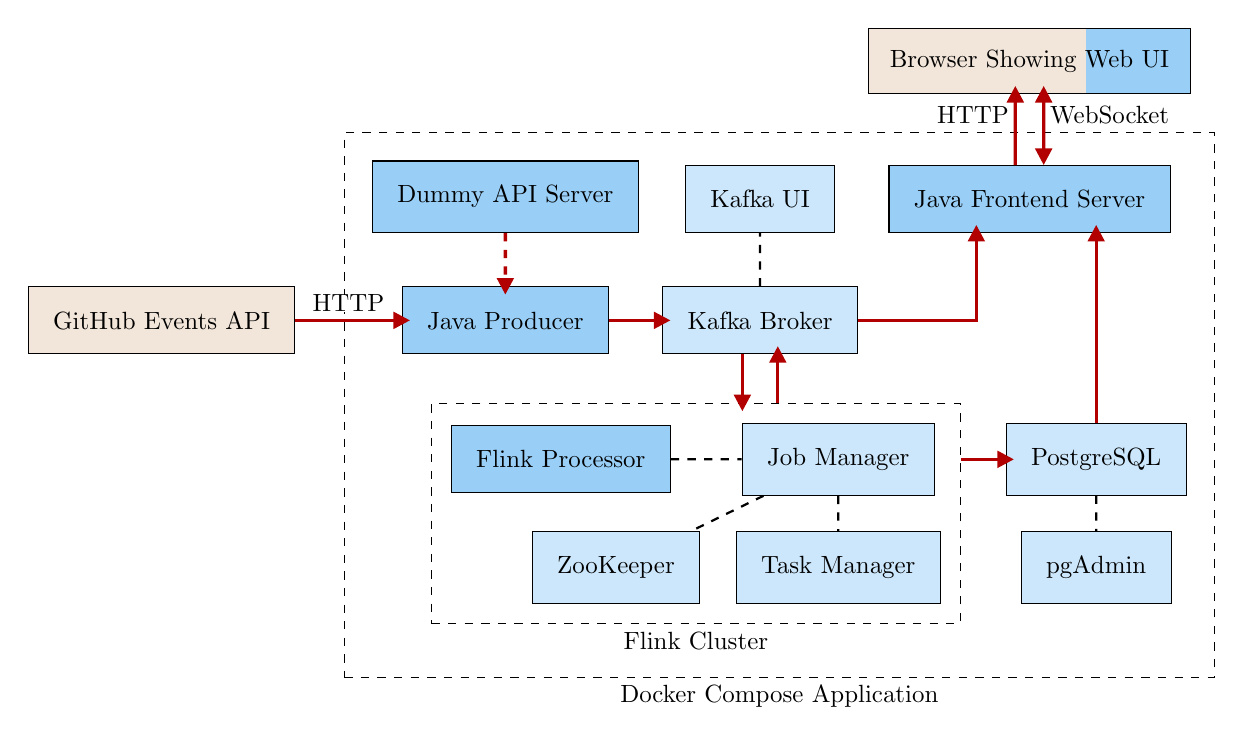
\begin{tikzpicture}[scale=0.9, transform shape]
    \node[external] (github) {GitHub Events API};
    \node[build, right=1.5 of github] (producer) {Java Producer};
    \draw[flow] (github) -> (producer) node [midway, fill=white, above=0.1] {HTTP};
    \node[internal, right=0.75 of producer] (kafka) {Kafka Broker};
    \draw[flow] (producer) -> (kafka);
    \node[internal, above=0.75 of kafka] (kafkaui) {Kafka UI};
    \draw[dashed, thick] (kafka) -> (kafkaui);
    \node[build, below=of kafka, xshift=-80] (processor) {Flink Processor};
    \node[internal, right=of processor] (jobmanager) {Job Manager};
    \draw[dashed, thick] (processor) -> (jobmanager);
    \node[internal, below=0.5 of jobmanager] (taskmanager) {Task Manager};
    \draw[dashed, thick] (jobmanager) -> (taskmanager);
    \node[internal, left=0.5 of taskmanager] (zookeeper) {ZooKeeper};
    \draw[dashed, thick] (jobmanager) -> (zookeeper);
    \begin{scope}[on background layer]
      \node[draw, dashed, fit=(processor)(jobmanager)(taskmanager), inner sep=7] (flink) {};
      \node[below=0.1 of flink] (flinklabel) {Flink Cluster};
    \end{scope}
    \draw[flow] ($(kafka.south)-(0.25,0)$) -> ($(kafka |- flink.north)-(0.25,0)$);
    \draw[flow] ($(kafka |- flink.north)+(0.25,0)$) -> ($(kafka.south)+(0.25,0)$);
    \node[build, above=0.75 of producer] (dummy) {Dummy API Server};
    \draw[flow, dashed] (dummy) -> (producer);
    \node[build, right=0.75 of kafkaui] (frontend) {Java Frontend Server};
    \draw[flow] (kafka) -| ($(frontend.south)-(0.75,0)$);
    \node[internal, right=of jobmanager] (postgres) {PostgreSQL};
    \node[internal, below=0.5 of postgres] (pgadmin) {pgAdmin};
    \draw[dashed, thick] (postgres) -- (pgadmin);
    \draw[flow] ($(postgres -| flink.east)$) -> ($(postgres.west)$);
    \draw[flow] ($(postgres.north)$) -> ($(postgres |- frontend.south)$);
    \node[mixed, above=of frontend] (browser) {Browser Showing Web UI};
    \draw[flow] ($(frontend.north)-(0.2,0)$) -> ($(browser.south)-(0.2,0)$) node [midway, fill=white, above left=0.1] {HTTP};
    \draw[biflow] ($(frontend.north)+(0.2,0)$) -> ($(browser.south)+(0.2,0)$) node [midway, fill=white, above right=0.1] {WebSocket};
    \begin{scope}[on background layer]
      \node[draw, dashed, fit=(flink)(flinklabel)(producer)(kafkaui)(frontend)(dummy)(postgres), inner sep=10] (docker) {};
      \node[below=0.1 of docker] (dockerlabel) {Docker Compose Application};
    \end{scope}
  \end{tikzpicture}
  \caption{Implemented application architecture. Blue indicates parts of the architecture controlled by the project, while the brown indicates external components. Darker blue represents components implemented as part of the project, while light blue components represent the use of existing software that has merely been configured.}
  \label{fig:arch}
\end{figure*}


\subsubsection{Data Ingestion}
A custom Kafka Producer is responsible for interfacing with the GitHub Events API. It polls the GitHub Events API at a configurable interval and depth. The code is implemented to respect GitHub's rate limiting, automatically pausing if the limit is hit. To capture all events, the polling retrieves overlapping windows of events with subsequent polls. Therefore, after receiving the list of events from the GitHub API, this component will also handle deduplication of events. For this task, the producer maintains a cache of the most recent event IDs. The producer then publishes the deduplicated raw GitHub events as JSON serialized strings to a dedicated Kafka topic, called \inlinecode{raw_events}.

During real deployment of the application, it is intended that the producer polls from the official GitHub API. However, for testing and development purposes a dummy API server has been developed. It offers the same \inlinecode{/events} endpoint, but does not require a real access token and has configurable throughput. The producer interacts with it in the same way as the official API.

\subsubsection{Stream Processing}
The core processing on the events is performed in a custom Apache Flink job. It is used to process the stream of events to extract relevant information and compute various aggregations to derive meaningful analytics. It consumes raw events from the \inlinecode{raw_events} Kafka topic, performs several complex processing operations. The transformations performed are organized into a series of modular pipelines, each responsible for feeding one table in PostgreSQL and one topic in Kafka. The following subsections discuss the main processing steps performed in the Flink based processor.

\paragraph{Preprocessing and Time Management} \label{preproc}
The first step in the processing pipeline is to parse the raw JSON events. The job operates in event time by assigning as timestamp the \inlinecode{created_at} timestamp extracted from the JSON payload. A watermark strategy tolerating up to 10 seconds of out-of-orderness is applied. Late events beyond this window are handled via specific allowed lateness strategies depending on the window type of different later operations.

Events are then passed on to subsequent steps, one of which parses the event payloads and generates human-readable descriptions, e.g., \inlinecode{"Roland pushed 3 commits to repo"}. It then takes this description, together with the event kind, the repository ID, and the user ID, as an output. These processed events are what is used in the frontend client to implement the live events stream.

\paragraph{User and Repository Information}
Not all events involving a specific user or repository contain all information about the concerning entry. For example, in some cases we only get information about the user ID, and are missing the rest of the user information. To improve the user interface, the processor therefore contains some transformations for extracting and aggregating user and repository details. For each event, we extract from the payload all the user and repository details.

Since events often contain only partial information about an entity, these extracted details have to be merged on a per-field basis, as compared to the full row, as is done with the other computation results generated by the Flink job. To handle this, these pipelines assign per-field sequence numbers to each update. The downstream database sink uses these sequence numbers to ensure that only that part of a row is updated for which incoming data is strictly newer than what is currently stored. A similar merging is applied on the frontend client using the real-time updates it receives.

\paragraph{Windowed Aggregation}
For historical data display, primarily for the charts in the frontend UI, the processor job performs windowed aggregation. It uses standard Flink Tumbling Windows of 10 seconds and 5 minutes duration to build long-term history of event counts. Event counts are computed for multiple different groupings. First, event count aggregations are computed on a per-type basis. Further, they are also computed per-user and per-repository. Finally, in addition to the total event count, for repositories the job also computes the count of new stars, which is used as an input to the trending score computation.

For real-time counters, standard sliding windows as provided by Flink proved too inefficient. Instead, the system uses a custom operator. This operator maintains circular buckets to aggregate counts efficiently across multiple overlapping window sizes of 5 minutes, 1 hour, 6 hours, and 24 hours simultaneously. This allows the dashboard to show the events in the last 24 hours updated every second without the overhead of maintaining millions of window objects.

\paragraph{Ranking and Trending}
To generate the user and repository rankings, the process consumes the output of the real-time counters. A custom operator is used to compute and maintain the complete ranking for each category. However, outputting the complete ranking, or even just the rows that have shifted, for each time a live counter changes, would be prohibitively expensive. Instead, the operator simply outputs an update including only the row for which the count changed. However, crucially, the updates produced by the operator include both the new and the old row number, allowing the frontend client to locally reconstruct exactly how the ranking changed.

For the global lists of trending repositories, the number of new stars is used. A custom operator calculates a composite score by combining new star counters across different time horizons, allowing the system to flag repositories experiencing a sudden surge in interest. The trending score is computed as
\begin{align*}
    t_\mathrm{score} = 10 s_{5\mathrm{m}} + 5 s_{5\mathrm{h}} + 2 s_{6\mathrm{h}} + s_{24\mathrm{h}} ,
\end{align*}
where $s_t$ is the number of new stars the repository has received in the latest time window of length $t$. This is a relatively simplistic model, but works reasonably well to identify trending repositories. By assigning a higher weight to more recently obtained stars, repositories that are experiencing immediate popularity are weighted more highly, but long term popularity is still taken into account.

\paragraph{Output of Results}
After performing the processing steps to compute the different analytics, the results are first written to PostgreSQL tables. Row updates are modeled as upserts, i.e., they represent an insert or an update of a single row. During this process each row is assigned a sequence number. This number is used by the client to know whether a row it receives from the frontend server is newer or older than the one it may already have. After writing the result to PostgreSQL, the row updates are sent to dedicated Kafka topics. Note that results are sent to Kafka only after they have been committed into PostgreSQL. 
This sequence ensures data consistency. By committing to PostgreSQL before Kafka, the system prevents a race condition where a frontend snapshot read from the database might miss updates already broadcast over the Kafka stream. After outputting the results to PostgreSQL and Kafka, they are ready to be consumed by the frontend.

\subsubsection{Data Serving}
A Java-based server acts as a bridge between the backend and the frontend client. It serves static assets and hosts a WebSocket endpoint. The processed data from Flink, that has been published to PostgreSQL tables and Kafka topics, is made available to the frontend client via a WebSocket API. It combines data queried from Postgres with real-time streams consumed from Kafka. The way this works is that the frontend client can request either reads from the table, or subscribe to a specific table with filters. In case of a table read, the frontend server connects to PostgreSQL and then forwards the results to the client. For real-time updates, the frontend server connects to all Kafka topics when starting the server, avoiding having to open a separate Kafka consumer for each client. Then, for each event it receives from Kafka, finds all clients that currently have a subscription matching the event, forwarding the event to those clients.

\subsubsection{Frontend}
The user interface is implemented as a custom single-page application using React and React Router, served by the frontend server. It offers an interactive dashboard with dynamic charts that update in real time as new data arrives. To obtain the real-time data, it connects via WebSocket to the frontend server. Upon connection, it subscribes to live updates, and then requests an initial snapshot from the backend, which is sourced from the DB. Doing it in this order ensures that no events are missed, and the sequence numbers are used to ensure new rows are not overwritten with old ones. As new messages arrive via WebSocket, the charts and counters increment in real time.

\subsubsection{Storage}

The database serves two purposes. Firstly, it is required for providing initial state for the dashboard, without having to wait for all values to update or replaying old events from Kafka. Second, it enables the retrieval of historical results. The database contains a table for each of the aspects computed by the Flink process, such as the events stream, the user and repository details, as well as the live and historical aggregations of event counts. TimescaleDB hypertables are used for some tables for automatic partitioning and using a retention policy to delete old data.

For the rankings, virtual views are used to compute row numbers and ranks based on the live scores. These are virtual views instead of proper tables because the high frequency of updates causes the rankings to change frequently. Since the change of a single row in the live scores could cause a cascade of row changes, using a materialized table would lead to unsustainable update volumes. These are two views to ensure low-latency queries for the frontend. One that is faster when retrieving a range of rows, and one that is faster for querying a very small number of rows. The frontend server dynamically switches between these for best performance.

\subsubsection{Messaging}

The final component of the architecture is formed by Apache Kafka. Kafka serves to decouple the ingestion from the processing, as well as the processing from the serving of the transformation results in the frontend. In addition to a topic used for the stream of raw events generated by the processor, the architecture utilizes specific topics for each of the outputs generated by the Flink processor. The Flink processor publishes processed results to these output topics for the frontend to consume in real time.

\subsection{Scalability and Reliability}

The system is designed for both resilience and scalability and efficiency.

\paragraph{Fault Tolerance}
Flink is configured to take incremental checkpoints of the RocksDB backend. In the event of a TaskManager failure, the job restarts from the last checkpoint, ensuring at-least-once processing semantics of the pipeline. At-least-once semantics are acceptable for this project, since all the outputs of the Flink processor are handled as upserts to the tables. Additionally, Flink has also been configured for high availability with the help of a ZooKeeper container. This means that the system is able to recover from JobManager failure, allowing jobs to restart from the last checkpoint using the metadata stored in ZooKeeper.

Further, if the processing layer goes offline for maintenance or unexpected failure, Kafka retains the message log. Upon restart, Flink processes the backlog to catch up. If however the producer goes down, events will be lost. This is unavoidable because the GitHub Events API does not offer any way to acquire older events than the last 300. One way to mitigate the issue would be by running multiple producers in parallel. This would cause duplicate events to be written to Kafka, but this would be acceptable since there is an additional deduplication step in the Flink processor.

\paragraph{Handling Out-of-Order Data}
As discussed in \Cref{preproc}, a watermark strategy tolerating up to 10 seconds of out-of-orderness is applied in the Flink processor. For the historical windowed aggregations, a specific lateness, 50 minutes for 5-minute windows and 100 seconds for the 10-second window, is additionally allowed for late-arriving events. This will cause an update to previously emitted window results, ensuring eventual consistency. A similar approach is taken for the live window aggregations. Here late events are used only to update the most recently emitted window, and any window emitted in the future.

For row updates in the frontend client, simply applying the latest arriving event is incorrect because the results of the snapshot replay may arrive after the real-time updates from the subscription. To solve this issue, the system assigns a sequence number at the ingestion point before the database sink. The client then only considers the latest version of each row by dropping events that arrive late with an earlier sequence number.

\paragraph{Scalability}
To improve scalability of the application, the Kafka topics are partitioned, allowing the Flink job to scale out its parallelism. Furthermore, most operators in the Flink processing job, such as parsing, windowing, mapping are fully parallel.

However, there are some limitations to the parallelism in the Flink processor. Global ranking requires gathering data to a single node to compare with all other values, which represents a theoretical bottleneck. Though sufficient for the current volume of GitHub data, this is an aspect of the architecture that is currently not scalable. Note that parallelization is still possible between the different rankings, i.e., ranking per-user and per-repository activity can be computed independently in parallel. Similarly, the rankings for different time window lengths can be computed in parallel.



\section{Functionalities} \label{functionalities}

The user interface is designed to be intuitive while displaying high-density information. This section will go through the key functionalities provided to user, illustrated with screenshots of the application.

\subsection{Live Dashboard}

\begin{figure}[ht]
    \centering
    \includegraphics[width=\linewidth]{figures/dashboard.png}
    \caption{Example screenshot of the main dashboard of the application. At the top, right below the header, are the per-kind event counter. Below to the right is the filterable stream of live events and on the left are the user and repository rankings.}
    \label{fig:dash}
\end{figure}

Users start at the home page, which represents the main dashboard for the application. It shows a number of different components to provide an overarching view. An example screenshot depicting the user interface of the dashboard can be seen in \Cref{fig:dash}.

\paragraph{Live Event Stream}
A scrolling feed of the latest events is shown on the bottom right of the dashboard. Each event is parsed into a human-readable description in the Flink processor, and these descriptions are displayed here. Users can filter this stream by event kind, user, or repository, using the input fields right above the live feed.

\paragraph{Real-Time Event Counters}
Dynamic counters display the total volume of specific event types, e.g., commits, opened or closed issues, or new forks, over sliding windows at the top of the dashboard. The duration of the sliding window is configurable to either 5 minutes, 1 hour, 6 hours, or one day. In all cases they are updated once a second. Next to the counters the UI also displays a chart showing the evolution of the volume over the selected time window.

\subsection{Activity Leaderboards}

\begin{figure}[ht]
    \centering
    \includegraphics[width=\linewidth]{figures/leaderboard.png}
    \caption{Example screenshot of the leaderboards on the main dashboard. On the left are the user rankings, while on the right we see the repository rankings.}
    \label{fig:board}
\end{figure}

Still on the main dashboard, the application also maintains continuously updated rankings over users and repositories as shown in \Cref{fig:board}. Users can be ranked by the number of events they generated. Repositories can also be ranked by the volume of activity, but they can additionally be ranked also by either the trending score or the raw number of stars. All rankings, except for the trending score that already combines all window lengths, it is possible for the user to select the length of sliding window for which the ranking is to be shown. Like for the per-kind counter, also the ranking shows a chart to illustrate the evolution over the selected window.

The trending score highlights repositories rapidly gaining popularity. This is calculated using a linear combination of new stars over multiple time windows, allowing the system to detect viral trends faster than simple daily counts, while being less noisy than simply using the 5-minute counts.

\subsection{Detailed Pages} \label{details}

Beyond the main dashboard, specific views allow for deeper analysis. These can be navigated through from the main dashboard either through the search functionality, clicking the real-time event counter cards, or by using one of the links in the leaderboards or event stream.

\begin{figure}[ht]
    \centering
    \includegraphics[width=\linewidth]{figures/events.png}
    \caption{Example screenshot of the event page. Historical counts for the selected event kind at the top, with distribution of events over time or the last hour at the bottom.}
    \label{fig:events}
\end{figure}

\paragraph{Events Page}
Firstly, there is a page dedicated for each event kind. An example of such a page is shown in \Cref{fig:events}. This page provides insights into specific types of events and the distribution among event types. At the top of the page, it includes an area chart showing how the volume for the selected event kind changed over time. Additionally, the page includes a pie chart showing the distribution of event types over the last hour and stacked area charts for historical trends at the bottom of the page. A user may click on one of the slices of the pie, or areas of the chart, to quickly switch to the dedicated view for that event type. This will affect the area chart shown at the top.

\begin{figure}[ht]
    \centering
    \includegraphics[width=\linewidth]{figures/repo.png}
    \caption{Example screenshot of the dedicated repository page. General repository information is shown at the top. Below that the rankings by different time windows and metrics and at the very bottom the historical activity and new stars.}
    \label{fig:repo}
\end{figure}

\paragraph{Repository Page}
A page dedicated to each individual repository is also provided as depicted in \Cref{fig:repo}. The page includes, in addition to some general information about the repository such as a link to GitHub, a description, or a link to the owner, also per-repository statistics. It shows the rank of the repository in the global activity and new stars leaderboards for all available time windows. Further, included is also a historical chart of event counts and one of new stars.

\begin{figure}[ht]
    \centering
    \includegraphics[width=\linewidth]{figures/user.png}
    \caption{Example screenshot of the dedicated user page. General user information is show at the top. Below that the rankings by different time windows and at the bottom the historical activity.}
    \label{fig:user}
\end{figure}

\paragraph{User Page}
Similar to the repository page, details for a specific user's activity history and their global ranking based on contribution volume are shown in a dedicated page. \Cref{fig:user} shows an example screenshot of that page. Again, it includes in addition to the computed statistics also some general information about the user, such as the avatar and whether the user is a bot or a regular user account.

\subsection{Search Functionality}

\begin{figure}[ht]
    \centering
    \includegraphics[width=\linewidth]{figures/search.png}
    \caption{Example screenshot of the search bar. Shows results for the search of \inlinecode{"rolandbe"}, including some found users and some repositories.}
    \label{fig:search}
\end{figure}

A global search bar is provided at the top of all pages as shown in \Cref{fig:search}. The search bar allows the user of the application to quickly search for specific users and repositories based on user or repository name. This enables the application to be used also for analyzing individual user and repositories, which would otherwise be very hard to find if they are not at the top of the leaderboards. Clicking on one of the search results navigates the user directly to the relevant detail page described in \Cref{details}.



\section{Lessons Learned} \label{leasons}

This section concludes the report by discussing what has worked well in the project, what were some of the main challenges, and what future improvements could be made to the system.

\subsection{Successes}

Overall, the architecture proved robust for the defined use case. The combination of Kafka and Flink handled the throughput of the GitHub API relatively well, even on somewhat older hardware. The use of Docker Compose significantly simplified the deployment process, by making the complex distributed system reproducible on different machines. The integration of TimescaleDB allowed for efficient storage and querying of historical time-series data without the operational overhead of managing a separate time-series database. The resulting dashboard provides a window into the development activity of the open-source world.

\subsection{Challenges}

Even with these successes, the project still faced some challenges.

\paragraph{Real-Time Ranking}
Generating a global leaderboard that updates in real-time was non-trivial. The main difficulty arises from the fact that a large number of ranks can change quickly. For example, if a repository jumps up in the ranking, all rows below may also be moved. Achieving this efficiently required tight coordination between the ranking process in Flink, the view based optimizations in the database, and the ability of the frontend to handle ranking updates in a specialized way.

\paragraph{High-Frequency Updates for Long Windows}
Standard Flink windowing proved inefficient for maintaining sliding windows that are very long, e.g., 24 hours, but are updated very frequently, e.g., every 1 second. This necessitated the implementation of a custom \inlinecode{KeyedProcessFunction} to optimize state management and triggering.

\paragraph{API Changes}
During the development lifecycle, specifically around October, GitHub modified their API payload, removing certain details. This caused the processing to crash, requiring refactoring of some parts of the parsing and transformation logic in the Flink processor.

\paragraph{Debugging Flink}
Gaining sufficient visibility into the internal state of Flink operators during streaming execution was difficult. This made it difficult to diagnose logic errors in the complex windowing functions and ranking logic. Further, there was a problem with state continually growing in size that was hard to debug due to Flink's limited facilities of inspecting state.

\subsection{Potential Improvements}

The project also features multiple potential avenues for future improvements. Aside from adding additional charts using the existing analysis results, the following may be promising additions.

\paragraph{Enhanced Trending Algorithm}
The current trending score is a linear combination of star counts and as such very simplistic. A more sophisticated model could incorporate the acceleration of stars or social signals such as created issues, pull requests, or comments. This could help to identify trending repositories earlier.

\paragraph{Data Enrichment}
Integrating additional data sources, such as tracking mentions of repositories on social media such as X or Reddit, would also provide a more comprehensive view of the trending status of repositories. This information could be useful both to identify which repositories are trending but also possibly give insights into why they are trending, something that is currently obscured in the system.

\paragraph{Sentiment Analysis}
Finally, analyzing the text content of some types of the events, such as commit messages, issue descriptions, and pull request comments could provide qualitative insights into the sentiment of different developer communities.


\printbibliography

\end{document}
